\documentclass[
	a4paper,     		%% Papiergroesse: A4
	twoside,     		%% Zweiseitiges Layout (alternativ: oneside)
	headsepline, 		%% Horizontale Linie unter Kopfzeile
	footsepline, 		%% Horizontale Linie ueber Fusszeile
	titlepage,   		%% Eigenstaendige Titelseite (alternativ: notitlepage)
%	halfparskip, 		%% Halbe Leerzeile zwischen zwei Abschnitten (alternativ: parskip, ...)
	12pt,        		%% Schriftgroesse: 12pt (alternativ: 10pt, 11pt, ...)
%	bibtotoc,			%% Bibliographie in's Inhaltsverzeichnis aufnehmen
%	liststotoc,			%% Indexe in's Inhaltsverzeichnis aufnehmen
%	smallheadings,		%% Kleine Ueberschriften
%	DIV1,				%% Divisor, Zeilenl�nge ca. 70 Zeichen
%	draft			  	%% Entwurfsmodus, volle/leere Boxen markieren
%	abstracton			%% Titel "`Zusammenfassung"' einschalten
]{scrartcl}

%%%
%%% Pakete
%%%

%%% Grafik
%\usepackage{pstricks}

%%% Deutsche Sprache verwenden
%\usepackage{ngerman}

%%% Kodierung der Eingabezeichen setzen (fuer dt. Umlaute etc.)
\usepackage[ansinew]{inputenc}

%%% Zeichen-Kodierung in PDF-Dokumenten
\usepackage[T1]{fontenc}
%\usepackage{ae,aecompl}

\usepackage[T1]{url}
%%% ... und in tt-Font
\urlstyle{tt}

%%% amsmath, amssymb, amstext: Unterstuetzung div. mathematischer Zeichen etc.
%\usepackage{amsmath,amssymb,amstext}
\usepackage{eurosym}

%%% pifont: "pifont Xs and Check Marks"
%\usepackage{pifont}

%%% PostScript-Fonts ersetzen
\usepackage{psfrag}

%%% Programmcode einbinden, Listings
%\usepackage{listings}

%%% Farb-Unterstuetzung
\usepackage{color}

%%% Tabellen
\usepackage{booktabs}
\usepackage{array}
\usepackage{multirow}
\usepackage{tabularx}
\usepackage{threeparttable}	% Fussnoten in table-Umgebung

%%% Floats strikter positionieren (Option 'H'ere)
\usepackage{float}

%%%
%%% Pakete konfigurieren, Definitionen
%%%

%%% Ueberschriften bis zur Ebene 3 nummerieren
\setcounter{secnumdepth}{3}

%%% Neue Spaltentypen definieren
\newcolumntype{N}{>{\bfseries\scriptsize}l}
\newcolumntype{V}[1]{
	>{\bfseries\scriptsize\raggedright\hspace{0pt}}p{#1}
}

%%%
%%% Seitenlayout, Schriften
%%%

%%% scrpage2: KOMA Kopf- und Fusszeile
\usepackage[automark]{scrpage2}

%%% EM unterstrichen darstellen
%\usepackage{ulem}

%%% Schrift fuer Captions verkleinern
\setkomafont{captionlabel}{\scriptsize}
\setkomafont{caption}{\usekomafont{captionlabel}}

%%% Schrift fuer Ueberschriften umstellen
%\setkomafont{sectioning}{\normalcolor\bfseries}

%%% Schriften fuer Titel- und Fusszeile umstellen
%\setkomafont{pagehead}{\normalfont\sffamily}
\setkomafont{pagenumber}{\normalfont\rmfamily\slshape}

%%% Part-Ueberschrift nicht fett drucken
%\addtokomafont{part}{\mdseries}
%\addtokomafont{partnumber}{\mdseries}

%%% Default-Platzierungsbeschraenkungen aendern,
%%% s. http://www.dante.de/faq/de-tex-faq/html/makros2.html#1
\makeatletter
	\renewcommand{\fps@figure}{htbp}
	\renewcommand{\fps@table}{htbp}
\makeatother

%%%
%%% PDF-Einstellungen
%%%

%%% Fallunterscheidung: PDF- oder 'normale' Erstellung?
\usepackage{ifpdf}

%%% Falls wir PDF erzeugen...
\ifpdf
  %%% Serifenlose Schriften benutzen
  \usepackage{mathpazo}
  \usepackage[scaled=.95]{helvet}
  \usepackage{courier}	
  \renewcommand{\familydefault}{\sfdefault}
  \usepackage[sf]{titlesec}

  %%% Unterstuetzung fuer Grafiken
  \usepackage[pdftex]{graphicx}
 
  %%% Kompressionslevel: 0-9
  \pdfcompresslevel=9

  %%% Hyperlinks in PDF-Dokumenten
  \usepackage[%
  	pdftex,
    pagebackref=false,		%% Seitenzahlen der Quellseite(n) in Bibliographie auflisten? (true|false) 
    colorlinks=true,		%% Farblinks? (true -> Screen | false -> Print)    
    %%% PDF-spezifische Optionen
    bookmarks=true,			%% PDF-Bookmarks erstellen? (true|false)
    bookmarksopen=true,		%% Anfangs alle Bookmarks ausgeklappt anzeigen? (true|false) 
    bookmarksnumbered=true,	%% Abschnitt-Nummerierung in Bookmarks integrieren? (true|false)
    pdfstartpage={1},		%% Startseite beim Oeffnen der Datei
    pdfpagemode=UseOutlines,%% Anzeigemodus? (None|UseOutlines|UseThumbs|FullScreen)
    a4paper=true,			%% A4-Format
    breaklinks=false,
    linkcolor=gray			%% Link-Farbe
  ]{hyperref}

	%%% Dateiendung fuer Grafiken setzen -- so kann beim Einbinden der Grafik
	%%% auf die Endung verzichtet werden und es wird automatisch die korrekte 
	%%% Datei ausgewaehlt (.eps / .pdf)
  \DeclareGraphicsExtensions{.pdf}
  
  %%% Pfad fuer Bilder setzen
  \graphicspath{{./images}}

%%% ... oder im 'normalen' Modus sind
\else

  %%% Unterstuetzung fuer Grafiken
  \usepackage[dvips]{graphicx}

  %%% s.o.
  \DeclareGraphicsExtensions{.eps}
  \graphicspath{{./images}}

  %%% Hyperlinks in PS-Dokumenten, Optionen s.o.
  \usepackage[%
    dvips,
    colorlinks=false,
    breaklinks=true,				%% Duerfen Links umbrochen werden? (true|false)
  ]{hyperref}

\fi

%%% Informationen ueber das PDF-Dokument setzen
\hypersetup{
  pdftitle={4th Assignment},%
  pdfauthor={Jan Tammen (jan.tammen@htwg-konstanz.de)},%
  pdfsubject={System- und Software-Ergonomie},%
  pdfcreator={LaTeX with pdfeTeX},%
  pdfproducer={LaTeX with pdfeTeX},%
  pdfkeywords={SERG, 4th Assignment},%
%  pdfpagelayout=TwoColumnRight,
  pdffitwindow=true,
%  pdfstartview=FitH,
}

%%% Links im dvips-Mode auch umbrechen
%\usepackage{breakurl}

%%%
%%% Layout der Titelseite
%%%

%%% Titelkopf, erscheint oberhalb des Titels
\titlehead{
	\begin{figure}[H]
		\centering
		
\includegraphics[width=\textwidth]{../images/htwg-logo}
	\end{figure}
}

%%%% Subject, erscheint oberhalb des Titels
\subject{System- und Software-Ergonomie, WS 06/07}

%%% Titel
\title{4th Assignment}


%%%% Autor. Weitere Autoren mit \and{<Name>} hinzufuegen
\author{%
	Jan Tammen, 277143
}%

%%% Datum setzen
\date{\today}

%%% Rueckseite der Titelseite
\lowertitleback{%
	\footnotesize%
	Erstellt mit \LaTeXe\ unter Verwendung des \KOMAScript-Pakets.}

%%%
%%% Header und Footer
%%%
%\pagestyle{scrheadings}

%%%
%%% Beginn Hauptdokument
%%%
\begin{document}

%%% Titelseite erstellen
\maketitle

%%%
%%% Beginn Inhalt
%%%
\section{Task 5}
\subsection{Part 5a}
As an example of an embedded system, I want to present the ``Creative Zen 
Touch'' MP3 player. Its main purpose is, of course, playing music files. 
Additionally, you can use the player as a mobile storage device and put data 
files on it.

In figure \ref{fig:creative-zen-touch} the devive's user interface is shown. As 
we can see, there are 7 control buttons in total, plus a touch pad interface. 
On the left side, there are 2 buttons which relate to menu navigation and one 
which controls random playback functions. In the middle there is a 
``OK''-button for selecting files and the touch pad for scrolling through menus 
and file lists. Finally, there are 3 playback control buttons on the right 
side: rewind, play/pause and fast forward.

\begin{figure}
  \centering
  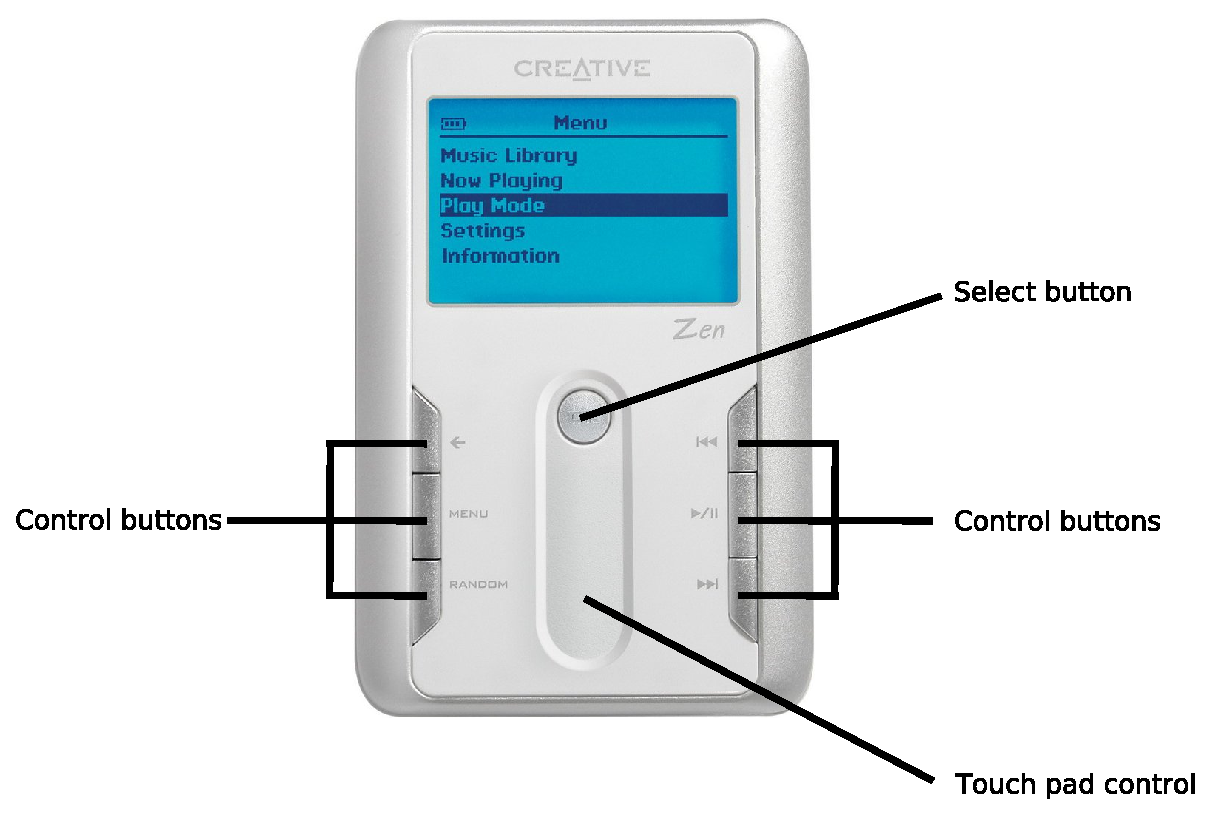
\includegraphics[width=1.00\textwidth]{../images/creative-zen-touch}
  \caption{User interface of the ``Creative Zen Touch''. Image: Creative Technology
  Ltd.}
  \label{fig:creative-zen-touch}
\end{figure}

Furthermore, there are two volume control buttons and the power switch on the 
player's left side, which is not shown here.

\subsection{Part 5b}
In the following sections I want to pick up three details of the player's
user interface and value them in terms of usability.

\subsubsection{Effectiveness}
While playing a song from a certain playlist you might be interested in the 
other artist's songs. So the player should offer a functionality to show and 
play the songs of the current track's artist.

Unfortunately, there is no such function -- if you want to play all songs of a 
specific artist, you have to leave your current playlist, go to the main menu 
and search for the artist manually.

\subsubsection{Efficiency}
If you have a very long list of songs in your player and you want to play a 
song whose title starts with a 'Z', you have to scroll all the way down the 
alphabetically sorted list until you find the song you are searching for. To 
shorten that search time, there is a 'search' included, which lets you choose 
the initial letter (from another list you have to scroll through) you want to 
jump to directly.

In my opinion this is a very ineffecient way to find a specific song.

\subsubsection{User Satisfaction}
In order to navigate the playlists or menus you have to use the integrated touch
pad device. The problem here is, that the touch pad is overly sensitive and that
makes selecting a certain entry quite difficult, at least at the beginning when
you are still ``untrained''. Although one can alter the pad's sensitivity, I 
think that even in the least sensitive mode you cannot navigate savely and 
select a specific list entry without ``oscilating'' between the entries above 
and below the target.

Another confusing aspect of the interaction controls is the fact that there is 
no ``stop playback'' button included, as figure \ref{fig:creative-zen-touch} 
already showed. So that actually breaks the principle of recognition, because 
audio playing devices usually have four playback controls: fast-forward, 
rewind, play/pause and stop.

\subsection{Part 5c}
To sum up, I have to say that I would rate the user interface's usability 
rather bad. There are a lot of glitches in the player's handling -- three of 
them mentioned in the sections above -- and that makes using ``special'' 
functions quite annoying. As long as you just play music in random mode and 
don't want to find specific songs or navigate through menus and change the 
sound settings, everything works okay.

\end{document}